\documentclass[12pt]{article}

% Use packages %
\usepackage{graphicx, courier, amsmath, amssymb, amscd, amsfonts, mathtools, bm, esint, leftidx, extarrows, latexsym, relsize, color, tikz, comment, stmaryrd}
\usepackage[obeyspaces]{url}% http://ctan.org/pkg/url

% Set length %
\setlength{\textwidth}{160mm}
\setlength{\textheight}{235mm}
\setlength{\oddsidemargin}{-0mm}
\setlength{\topmargin}{-10mm}

% Define h-bar %
\newsavebox{\myhbar}
\savebox{\myhbar}{$\hbar$}
\renewcommand*{\hbar}{\mathalpha{\usebox{\myhbar}}}

% Chinese input %
%\usepackage{xeCJK} 
%\setCJKmainfont{微軟正黑體}
%\usepackage[T1]{fontenc}
%\makeatletter

% Equation number %
%\@addtoreset{equation}{section} 
%\renewcommand\theequation{{\thesection}.{\arabic{equation}}}
%\makeatletter 

% Helper Command %
\newcommand{\argmin}{\operatornamewithlimits{argmin}}
\newcommand{\rmnum}[1]{\romannumeral #1} 
\newcommand{\Rmnum}[1]{\expandafter\@slowromancap\romannumeral #1@}
\newcommand{\overbar}[1]{\mkern 1.5mu\overline{\mkern-1.5mu#1\mkern-1.5mu}\mkern 1.5mu}
\makeatother
\newcommand*{\QEDA}{\hfill\ensuremath{\blacksquare}}
\newcommand*{\QEDB}{\hfill\ensuremath{\square}}
\newcommand*{\BmVert}{\bigm\vert}
\newcommand{\bigslant}[2]{{\raisebox{.2em}{$#1$}\left/\raisebox{-.2em}{$#2$}\right.}}
\newcommand{\Nelements}[3]{\left\{ #1, ~ #2, \ldots, ~ #3 \right\}}
\newcommand{\CBrackets}[1]{\left\{#1\right\}}
\newcommand{\SBrackets}[1]{\left[#1\right]}
\newcommand{\ParTh}[1]{\left(#1\right)}
\newcommand{\Ceil}[1]{\left\lceil#1\right\rceil}
\newcommand{\Floor}[1]{\left\lfloor#1\right\rfloor}
\newcommand{\BF}[1]{{\bf#1}}
\newcommand{\Inverse}[1]{{#1}^{-1}}
\newcommand{\Generator}[1]{\left\langle#1\right\rangle}
\newcommand{\AbsVal}[1]{\left|#1\right|}
\newcommand{\VecAbsVal}[1]{\left\|#1\right\|}
\newcommand{\BSlash}[2]{\left.#1\middle\backslash#2\right.}
\newcommand{\Divide}[2]{\left.#1\middle/#2\right.}
\newcommand{\SciNum}[2]{#1\times{10}^{#2}}
\newcommand{\Matrix}[2]{\ParTh{\begin{array}{#1}#2\end{array}}}
\newcommand{\MatrixTwo}[4]{\ParTh{\begin{array}{cc}{#1}&{#2}\\{#3}&{#4}\end{array}}}
\newcommand{\MatrixNByN}[1]{\Matrix{cccc}{{#1}_{11} & {#1}_{12} & \cdots & {#1}_{1n} \\ {#1}_{21} & {#1}_{22} & \cdots & {#1}_{2n} \\ \vdots & \vdots & \ddots & \vdots \\ {#1}_{n1} & {#1}_{n2} & \cdots & {#1}_{nn}}}
\newcommand{\ndiv}{\hspace{-4pt}\not|\hspace{2pt}}
\newcommand{\eqdef}{\xlongequal{\text{def}}}%
\newcount\arrowcount
\newcommand\arrows[1]{\global\arrowcount#1 \ifnum\arrowcount>0
\begin{matrix}\expandafter\nextarrow\fi}
\newcommand\nextarrow[1]{\global\advance\arrowcount-1 \ifx\relax#1\relax\else \xrightarrow{#1}\fi\ifnum\arrowcount=0 \end{matrix}\else\\\expandafter\nextarrow\fi}
\newcommand{\horrule}[1]{\rule{\linewidth}{#1}}

% Tikz settings %
\usetikzlibrary{shapes,arrows}
\tikzstyle{decision} = [diamond, draw, fill=white!20, text width=4.5em, text badly centered, node distance=3cm, inner sep=0pt]
\tikzstyle{block}    = [rectangle, draw, fill=white!20, text width=8em, text centered, rounded corners, minimum height=4em]
\tikzstyle{point}    = [fill = white!20, minimum size=0.5cm]
\tikzstyle{line}     = [draw, -latex']
\tikzstyle{mapsto}   = [draw, |->]
\tikzstyle{cloud}    = [draw, ellipse,fill=red!20, node distance=3cm, minimum height=2em]

\begin{document}

\baselineskip 6.5mm
\setlength{\parindent}{0pt}
\title{ 
\normalfont \normalsize 
\horrule{0.5pt} \\[0.4cm]
\huge { \Huge Machine Learning \\ \large Answer Sheet for Homework 4 }\\ % The assignment title
\horrule{2pt} \\ [0.5cm]
}
\author{ { \Large Da-Min HUANG } \\
{\small R04942045} \\
{\small\textit{Graduate Institute of Communication Engineering, National Taiwan University}}
}
\date{November 25, 2015}
%\allowdisplaybreaks[4]
\maketitle

\subsection*{Problem 1}

Deterministic error is the difference between best $h^* \in H$ and $f$. If $H^\prime\subset H$, then the complexity of $H^\prime$ is lower than $H$ in general. Hence, in general, the deterministic error increases.

\QEDB

\horrule{0.5pt}

\subsection*{Problem 2}

\begin{align}
H\ParTh{10,0,3}\cap H\ParTh{10,0,4}&=\CBrackets{\sum_{i=0}^{2}w_qL_q\ParTh{x}}\cap\CBrackets{\sum_{i=0}^{3}w_qL_q\ParTh{x}}\\
&=\CBrackets{\sum_{i=0}^{2}w_qL_q\ParTh{x}}=H_2
\end{align}
Hence, $Q=2$.
\begin{comment}
\begin{enumerate}
	\item
	\begin{align}
	H\ParTh{10,0,3}\cap H\ParTh{10,0,4}&=\CBrackets{\sum_{i=0}^{2}w_qL_q\ParTh{x}}\cap\CBrackets{\sum_{i=0}^{3}w_qL_q\ParTh{x}}\\
	&=\CBrackets{\sum_{i=0}^{2}w_qL_q\ParTh{x}}=H_2
	\end{align}
	\item
	\begin{align}
	H\ParTh{10,0,3}\cup H\ParTh{10,1,4}&=\CBrackets{\sum_{i=0}^{2}w_qL_q\ParTh{x}}\cup\CBrackets{\sum_{i=0}^{3}w_qL_q\ParTh{x}+\sum_{i=4}^{10}L_q\ParTh{x}}\\
	&=\CBrackets{\sum_{i=0}^{3}w_qL_q\ParTh{x}+\sum_{i=4}^{10}L_q\ParTh{x}}
	\end{align}
	\item
	\begin{align}
	H\ParTh{10,1,3}\cap H\ParTh{10,1,4}&=\CBrackets{\sum_{i=0}^{2}w_qL_q\ParTh{x}+\sum_{i=3}^{10}L_q\ParTh{x}}\cap\CBrackets{\sum_{i=0}^{3}w_qL_q\ParTh{x}+\sum_{i=4}^{10}L_q\ParTh{x}}\\
	&=\CBrackets{\sum_{i=0}^{2}w_qL_q\ParTh{x}+\sum_{i=4}^{10}L_q\ParTh{x}}
	\end{align}
	\item
	\begin{align}
	H\ParTh{10,0,3}\cup H\ParTh{10,0,4}&=\CBrackets{\sum_{i=0}^{2}w_qL_q\ParTh{x}}\cup\CBrackets{\sum_{i=0}^{3}w_qL_q\ParTh{x}}\\
	&=\CBrackets{\sum_{i=0}^{3}w_qL_q\ParTh{x}}=H_3
	\end{align}
\end{enumerate}
\end{comment}

\QEDB

\horrule{0.5pt}

\subsection*{Problem 3}

We have
\begin{align}
\BF{w}_{t+1}\leftarrow\BF{w}_{t}-\eta\nabla E_{\text{aug}}\ParTh{\BF{w}_t}
\end{align}
where $\nabla E_{\text{aug}}\ParTh{\BF{w}_t}$ is
\begin{align}
\nabla E_{\text{aug}}\ParTh{\BF{w}_t}=\dfrac{\partial}{\partial\BF{w}^T_t}\ParTh{E_{\text{in}}\ParTh{\BF{w}_t}+\dfrac{\lambda}{N}\BF{w}^T_t\BF{w}_t}=\dfrac{\partial E_{\text{in}}\ParTh{\BF{w}_t}}{\partial\BF{w}^T_t}+\dfrac{2\lambda}{N}\BF{w}_t
\end{align}
Hence, we have
\begin{align}
\BF{w}_{t+1}\leftarrow\ParTh{1-\dfrac{2\eta\lambda}{N}}\BF{w}_{t}-\eta\nabla E_{\text{in}}\ParTh{\BF{w}_t}
\end{align}

\QEDB

\horrule{0.5pt}

\subsection*{Problem 4}

Since $\BF{w}_{\text{lin}}$ is the optimal solution for the plain-vanilla linear regression, we have
\begin{align}
E_{\text{in}}\ParTh{\BF{w}_{\text{lin}}}\leq E_{\text{in}}\ParTh{\BF{w}_{\text{reg}}\ParTh{\lambda}}
\end{align}
Also, $\BF{w}_{\text{reg}}\ParTh{\lambda}$ is the optimal solution for $E_{\text{aug}}\ParTh{\BF{w}}$, we have
\begin{align}
E_{\text{aug}}\ParTh{\BF{w}_{\text{reg}}\ParTh{\lambda}}\leq E_{\text{aug}}\ParTh{\BF{w}_{\text{lin}}}
\end{align}
So, we have
\begin{align}
E_{\text{in}}\ParTh{\BF{w}_{\text{reg}}\ParTh{\lambda}}+\dfrac{\lambda}{N}\BF{w}^T_{\text{reg}}\ParTh{\lambda}\BF{w}_{\text{reg}}\ParTh{\lambda}&\leq E_{\text{in}}\ParTh{\BF{w}_{\text{lin}}}+\dfrac{\lambda}{N}\BF{w}^T_{\text{lin}}\BF{w}_{\text{lin}}\\
0\leq E_{\text{in}}\ParTh{\BF{w}_{\text{reg}}\ParTh{\lambda}}-E_{\text{in}}\ParTh{\BF{w}_{\text{lin}}}&\leq \dfrac{\lambda}{N}\ParTh{\VecAbsVal{\BF{w}_{\text{lin}}}^2-\VecAbsVal{\BF{w}_{\text{reg}}\ParTh{\lambda}}^2},~\forall\lambda
\end{align}
Hence, we have $\VecAbsVal{\BF{w}_{\text{lin}}}\geq\VecAbsVal{\BF{w}_{\text{reg}}\ParTh{\lambda}}$ if $\lambda>0$.

Since this inequality holds for all $\lambda$ and $\VecAbsVal{\BF{w}_{\text{lin}}}$ is not a function of $\lambda$. We know that $\VecAbsVal{\BF{w}_{\text{reg}}\ParTh{\lambda}}$ is a non-increasing function of $\lambda$ for $\lambda\geq0$.

\QEDB

\horrule{0.5pt}

\subsection*{Problem 5}

For constant model with three points $A\ParTh{-1,0}$, $B\ParTh{\rho,1}$ and $C\ParTh{1,0}$.
\begin{align}
\dfrac{1}{3}\ParTh{\underbrace{\ParTh{0-\dfrac{1}{2}}^2}_{\text{leave }A}+\underbrace{\ParTh{1-0}^2}_{\text{leave }B}+\underbrace{\ParTh{0-\dfrac{1}{2}}^2}_{\text{leave }C}}=\dfrac{1}{2}
\end{align}
For linear model. Leave $A$, we get line $y=\dfrac{1}{\rho-1}\ParTh{x-1}$; leave $B$, we get line $y=0$; leave $C$, we get line $y=\dfrac{1}{\rho+1}\ParTh{x+1}$. So the error is
\begin{align}
\dfrac{1}{3}\ParTh{\ParTh{0-\ParTh{\dfrac{-2}{\rho-1}}}^2+\ParTh{1-0}^2+\ParTh{0-\dfrac{2}{\rho+1}}^2}
\end{align}
Then we have
\begin{align}
\dfrac{1}{3}\ParTh{\dfrac{4}{{\rho^2-2\rho+1}}+1+\dfrac{4}{{\rho^2+2\rho+1}}}=\dfrac{1}{2}\Rightarrow\rho=\pm\sqrt{9+4\sqrt{6}}
\end{align}
Since $\rho>0$, we have $\rho=\sqrt{9+4\sqrt{6}}$.

\QEDB

\horrule{0.5pt}

\subsection*{Problem 6}

If the sender wants to make sure at least one person receives correct predictions on all 5 games. Then he should target at least 32 people at first game since there are half the number of people receive wrong prediction after each game and the sender can just ignore people who receives wrong prediction.

The sender sends
\begin{align}
32+16+8+4+2=62\text{ letters}
\end{align}
before the fifth game.

\QEDB

\horrule{0.5pt}

\subsection*{Problem 7}

From the conclusion above, we have
\begin{align}
1000-\ParTh{62+1}\times10=370
\end{align}

\QEDB

\horrule{0.5pt}

\subsection*{Problem 8}

All mathematical function derivated before looking at data is hypothesis set of size 1.

Take positive ray hypothesis set for example, it can generate $N$ possible models after given data. The function in this problem generated before given the data, so it must be some specific model instead of depending on some learning algorithm to learn from data.

Hence, the hypothesis set is of size 1.
\begin{comment}
The mathematical derivations with perfect prediction, which means the hypothesis set shatters the $N$ data. So the size of the hypothesis is $2^N$.
\end{comment}

\QEDB

\horrule{0.5pt}

\subsection*{Problem 9}

The Hoeffding bound is
\begin{align}
2M\exp\ParTh{-2\epsilon^2N}=2\exp\ParTh{-20000\times\ParTh{0.01}^2}=2e^{-2}\approx0.271
%2m_{\mathcal{H}}\ParTh{2N}\cdot2\exp\ParTh{-2\ParTh{\dfrac{\epsilon}{4}}^2N}=2^{20002}\exp\ParTh{-20000\ParTh{\dfrac{0.01}{4}}^2}
\end{align}

\QEDB

\horrule{0.5pt}

\subsection*{Problem 10}

The computation of Hoeffding bound is computated with data verified by $a\ParTh{\BF{x}}$. To improve the performance of $g\ParTh{\BF{x}}$, we should only give data sampled by $a\ParTh{\BF{x}}$.

Hence, if lucky enough, $a\ParTh{\BF{x}}\text{ AND }g\ParTh{\BF{x}}$ can improve the system.

\QEDB

\horrule{0.5pt}

\subsection*{Problem 11}

To get optimal solution, consider the following equation.
\begin{align}
&\nabla\ParTh{\sum_{n=1}^{N}\ParTh{y_n-\BF{w}^T\BF{x}_n}^2+\sum_{k=1}^{K}\ParTh{\tilde{y}_k-\BF{w}^T\tilde{\BF{x}}_k}^2}\\
=&-2\ParTh{\sum_{n=1}^{N}\BF{x}_n\ParTh{y_n-\BF{x}^T_n\BF{w}}+\sum_{k=1}^{K}\tilde{\BF{x}}_k\ParTh{\tilde{y}_k-\tilde{\BF{x}}^T_k\BF{w}}}\\
=&-2\ParTh{\ParTh{\BF{X}^T\BF{y}-\BF{X}^T\BF{X}\BF{w}}+\ParTh{\tilde{\BF{X}}^T\tilde{\BF{y}}-\tilde{\BF{X}}^T\tilde{\BF{X}}\BF{w}}}\\
=&~\BF{0}
\end{align}
Hence, we have $\BF{w}=\ParTh{\BF{X}^T\BF{X}+\tilde{\BF{X}}^T\tilde{\BF{X}}}^{-1}\ParTh{\BF{X}^T\BF{y}+\tilde{\BF{X}}^T\tilde{\BF{y}}}$.

\QEDB

\horrule{0.5pt}

\subsection*{Problem 12}

To minimize the formula, consider the following equation.
\begin{align}
\nabla\ParTh{\lambda\VecAbsVal{\BF{w}}^2+\VecAbsVal{\BF{X}\BF{w}-\BF{y}}^2}&=2\lambda\BF{w}+2\BF{X}^T\BF{X}\BF{w}-2\BF{X}^T\BF{y}=\BF{0}\\
\Rightarrow\BF{w}&=\ParTh{\BF{X}^T\BF{X}+\lambda\BF{I}}^{-1}\BF{X}^T\BF{y}
\end{align}
Hence, we have $\tilde{\BF{X}}=\sqrt{\lambda}\BF{I}$, $\tilde{\BF{y}}=\BF{0}$.

\QEDB

\horrule{0.5pt}

\subsection*{Problem 13}

$E_{\text{in}}=0.055$ and $E_{\text{out}}=0.052$.

\QEDB

\horrule{0.5pt}

\subsection*{Problem 14}

\begin{figure}[h]
	\centering
	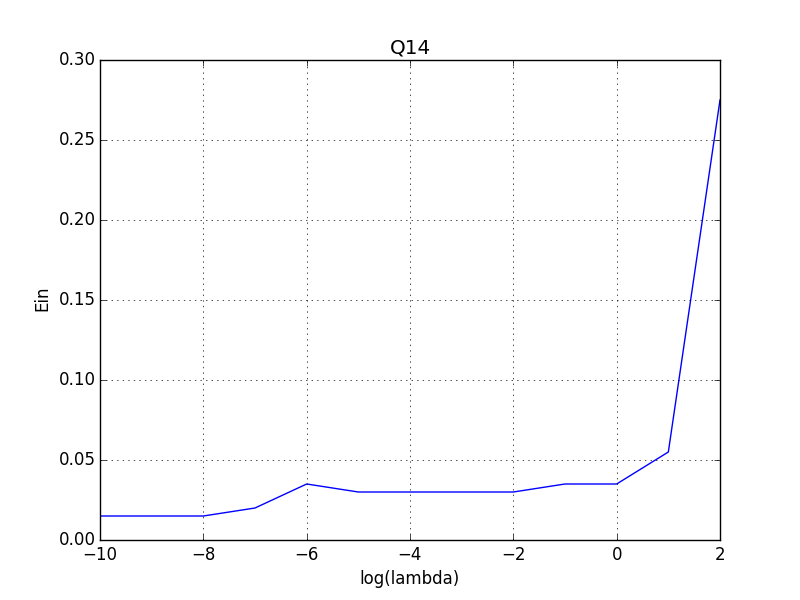
\includegraphics[scale=0.3]{Q14.png}
	\caption{Q14}
	\label{Q14}
\end{figure}
$\log_{10}\lambda=-8$, $E_{\text{in}}=0.015$ and $E_{\text{out}}=0.02$.
\begin{comment}
There are three lambda with minimal $E_{\text{in}}$.
\begin{enumerate}
	\item $\log_{10}\lambda=-10$, $E_{\text{in}}=0.015$ and $E_{\text{out}}=0.02$.
	\item $\log_{10}\lambda=-9$, $E_{\text{in}}=0.015$ and $E_{\text{out}}=0.02$.
	\item $\log_{10}\lambda=-8$, $E_{\text{in}}=0.015$ and $E_{\text{out}}=0.02$.
\end{enumerate}
\end{comment}

\QEDB

\horrule{0.5pt}

\subsection*{Problem 15}

\begin{figure}[h]
	\centering
	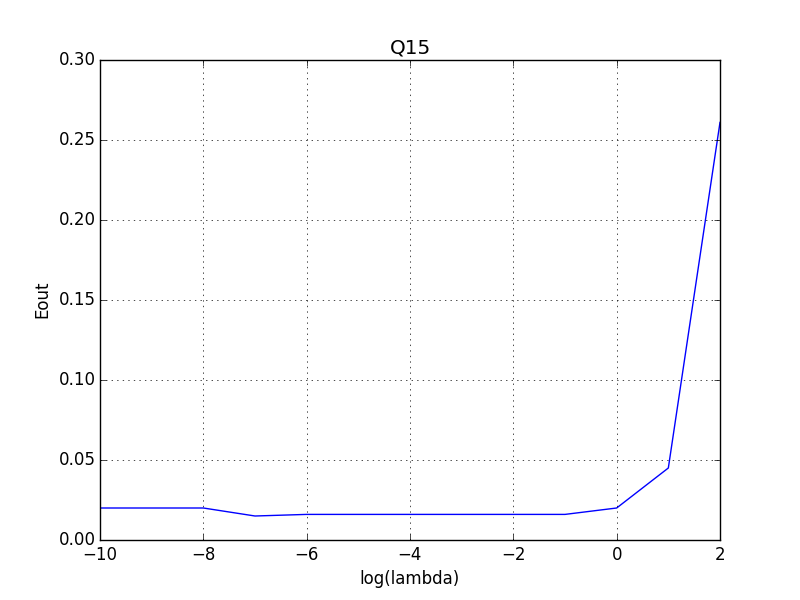
\includegraphics[scale=0.3]{Q15.png}
	\caption{Q15}
	\label{Q15}
\end{figure}
$\log_{10}\lambda=-7$, $E_{\text{in}}=0.03$ and $E_{\text{out}}=0.015$.

\QEDB

\horrule{0.5pt}

\subsection*{Problem 16}

\begin{figure}[h]
	\centering
	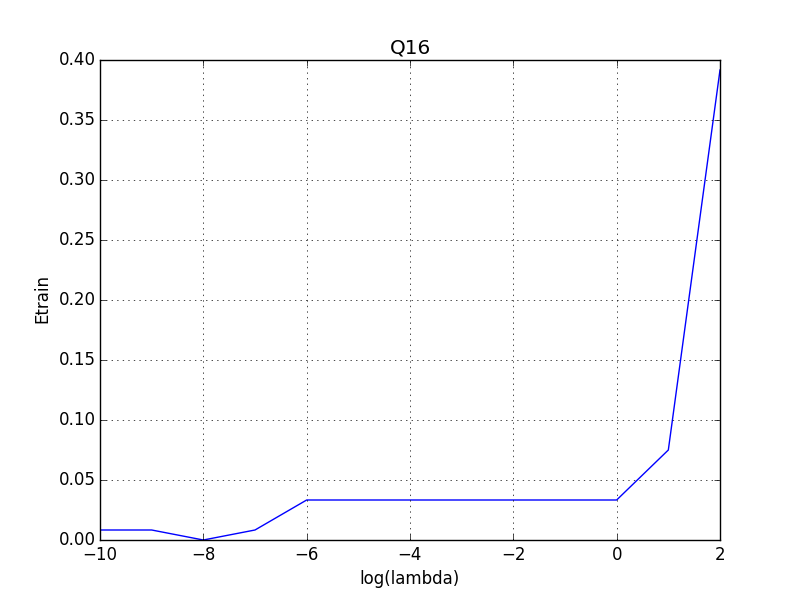
\includegraphics[scale=0.3]{Q16.png}
	\caption{Q16}
	\label{Q16}
\end{figure}
$\log_{10}\lambda=-8$, $E_{\text{train}}=0.0$, $E_{\text{val}}=0.05$ and $E_{\text{out}}=0.025$.
\begin{comment}
There are two lambda with minimal $E_{\text{in}}$.
\begin{enumerate}
	\item $\log_{10}\lambda=-9$, $E_{\text{train}}=0.0$, $E_{\text{val}}=0.1$ and $E_{\text{out}}=0.038$.
	\item $\log_{10}\lambda=-8$, $E_{\text{train}}=0.0$, $E_{\text{val}}=0.05$ and $E_{\text{out}}=0.025$.
\end{enumerate}
\end{comment}

\QEDB

\horrule{0.5pt}

\subsection*{Problem 17}

\begin{figure}[h]
	\centering
	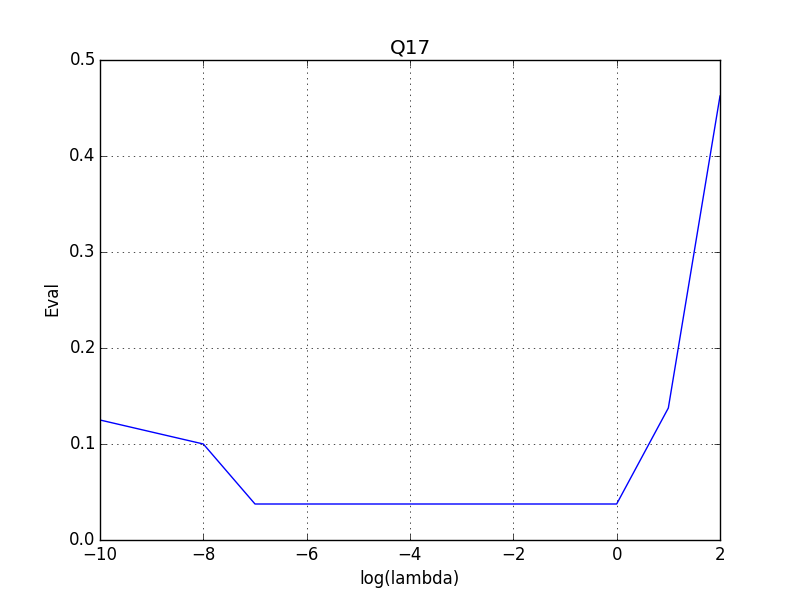
\includegraphics[scale=0.3]{Q17.png}
	\caption{Q17}
	\label{Q17}
\end{figure}
$\log_{10}\lambda=0$, $E_{\text{train}}=0.033$, $E_{\text{val}}=0.0375$ and $E_{\text{out}}=0.028$.
\begin{comment}
There are eight lambda with minimal $E_{\text{in}}$.
\begin{enumerate}
	\item $\log_{10}\lambda=-7$, $E_{\text{train}}=0.033$, $E_{\text{val}}=0.0375$ and $E_{\text{out}}=0.021$.
	\item $\log_{10}\lambda=-6$, $E_{\text{train}}=0.033$, $E_{\text{val}}=0.0375$ and $E_{\text{out}}=0.021$.
	\item $\log_{10}\lambda=-5$, $E_{\text{train}}=0.033$, $E_{\text{val}}=0.0375$ and $E_{\text{out}}=0.021$.
	\item $\log_{10}\lambda=-4$, $E_{\text{train}}=0.033$, $E_{\text{val}}=0.0375$ and $E_{\text{out}}=0.021$.
	\item $\log_{10}\lambda=-3$, $E_{\text{train}}=0.033$, $E_{\text{val}}=0.0375$ and $E_{\text{out}}=0.021$.
	\item $\log_{10}\lambda=-2$, $E_{\text{train}}=0.033$, $E_{\text{val}}=0.0375$ and $E_{\text{out}}=0.021$.
	\item $\log_{10}\lambda=-1$, $E_{\text{train}}=0.033$, $E_{\text{val}}=0.0375$ and $E_{\text{out}}=0.022$.
	\item $\log_{10}\lambda=0$, $E_{\text{train}}=0.033$, $E_{\text{val}}=0.0375$ and $E_{\text{out}}=0.028$.
\end{enumerate}
\end{comment}

\QEDB

\horrule{0.5pt}

\subsection*{Problem 18}

The returned $\log_{10}\ParTh{\lambda}=0\Rightarrow\lambda=1$. $E_{\text{in}}=0.035$ and $E_{\text{out}}=0.020$.

\QEDB

\horrule{0.5pt}

\subsection*{Problem 19}

\begin{figure}[h]
	\centering
	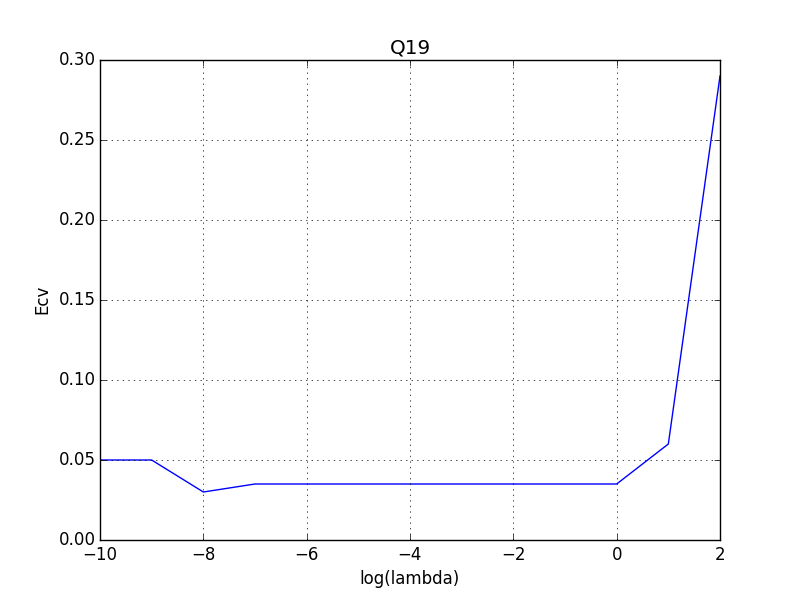
\includegraphics[scale=0.3]{Q19.png}
	\caption{Q19}
	\label{Q19}
\end{figure}
The returned $\log_{10}\ParTh{\lambda}=-8$ and $E_{\text{cv}}=0.03$.

\QEDB

\horrule{0.5pt}

\subsection*{Problem 20}

$E_{\text{in}}=0.015$ and $E_{\text{out}}=0.020$.

\QEDB

\horrule{0.5pt}

\subsection*{Problem 21}

To minimize the formula, consider the following equation.
\begin{align}
\nabla\ParTh{\lambda\VecAbsVal{\BF{\Gamma}\BF{w}}^2+\VecAbsVal{\BF{X}\BF{w}-\BF{y}}^2}&=2\lambda\BF{\Gamma}^T\BF{\Gamma}\BF{w}+2\BF{X}^T\BF{X}\BF{w}-2\BF{X}^T\BF{y}=\BF{0}\\
\Rightarrow\BF{w}&=\ParTh{\BF{X}^T\BF{X}+\lambda\BF{\Gamma}^T\BF{\Gamma}}^{-1}\BF{X}^T\BF{y}
\end{align}
Hence, we have $\tilde{\BF{X}}=\sqrt{\lambda}\BF{\Gamma}$, $\tilde{\BF{y}}=\BF{0}$.

\QEDB

\horrule{0.5pt}

\subsection*{Problem 22}

To minimize the formula, consider the following equation.
\begin{align}
\nabla\ParTh{\lambda\VecAbsVal{\BF{w}-\BF{w}_{\text{hint}}}^2+\VecAbsVal{\BF{X}\BF{w}-\BF{y}}^2}&=2\lambda\BF{w}-2\lambda\BF{w}_{\text{hint}}+2\BF{X}^T\BF{X}\BF{w}-2\BF{X}^T\BF{y}=\BF{0}\\
\Rightarrow\BF{w}&=\ParTh{\BF{X}^T\BF{X}+\lambda\BF{I}}^{-1}\ParTh{\BF{X}^T\BF{y}+\lambda\BF{w}_{\text{hint}}}
\end{align}
Hence, we have $\tilde{\BF{X}}=\sqrt{\lambda}\BF{I}$, $\tilde{\BF{y}}=\sqrt{\lambda}\BF{w}_{\text{hint}}$.

\QEDB

\horrule{0.5pt}

\section*{Reference}

\begin{enumerate}

\item[{[1]}] Lecture Notes by Hsuan-Tien LIN, Department of Computer Science and Information Engineering, National Taiwan University, Taipei 106, Taiwan.

%\item[{[2]}] Three proofs of Sauer-Shelah Lemma. (n. d. ). Retrieved Fall, 2010, from \url{http://www.cse.buffalo.edu/~hungngo/classes/2010/711/lectures/sauer.pdf}

\end{enumerate}

\end{document}